Neste capítulo mostraremos exemplos de resultados de utilização da ferramenta, para isso demonstraremos com alguns códigos simples a interação com o sistema e seus resultados, como também alguns exemplos de erros de montagem que são tratados neste projeto.

Para vermos melhores resultados, criamos os seguintes códigos,

\begin{itemize}
	\item Aritmética simples
	\item Sequência de fibonacci
\end{itemize}


\section{Possíveis erros de montagem}

	Como explicado na seção anterior, sendo a montagem, a parte que lida diretamente com a entrada do usuário, é necessário que o sistema saiba lidar com possíveis erros inseridos no código e devolver uma resposta adequada. Foram implementados as seguintes menasgens de erros,

	
	 Na figura \ref{fig:assemble_error_duplicated_symbol}, temos um exemplo de erro de declaração múltipla de símbolo, ou seja, se o programador declarar o mesmo símbolo em dois momentos diferentes no código.
	
	\begin{figure}[h!]
	  \centering
	  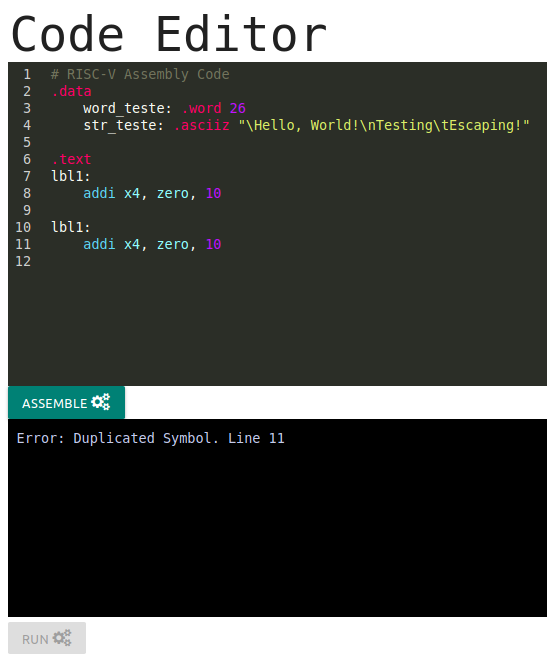
\includegraphics[width=8cm]{img/assemble_error_duplicated_symbol.png}
	  \caption{Erro de declaração múltipla de símbolo.}
	  \label{fig:assemble_error_duplicated_symbol}
	\end{figure}

	 Na figura \ref{fig:assemble_error_directives_strings}, temos um exemplo de erro da diretiva .asciiz ou .string, quando é declarado mais de uma string para um único símbolo.
	

	\begin{figure}[h!]
	  \centering	  
	  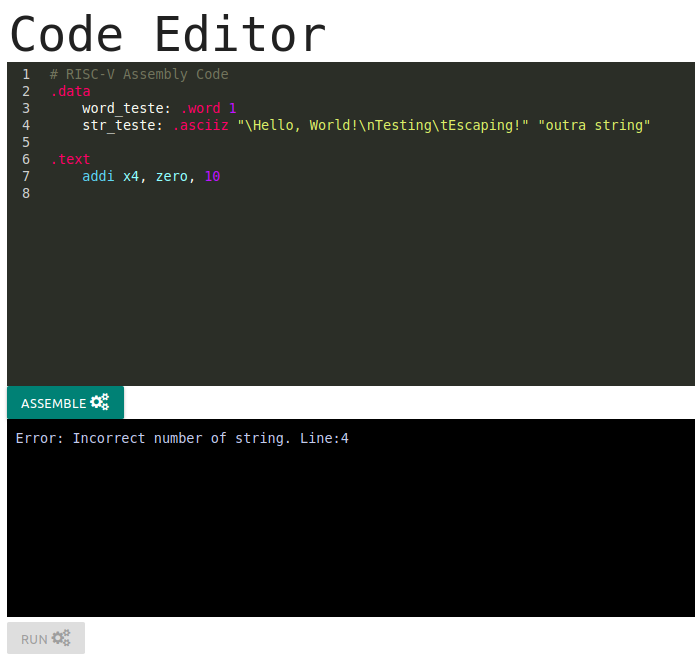
\includegraphics[width=8cm]{img/assemble_error_directives_strings.png}
	  \caption{Erro de declaração de diretiva string.}
	  \label{fig:assemble_error_directives_strings}
	\end{figure}


	 Na figura \ref{fig:assemble_error_imediato}, temos um exemplo de erro de valor de imediato, no caso deste projeto onde utilizamos tamanhos de palavra 32 bits, um valor superior a 4GB traria um overflow.
	
	\begin{figure}[h!]
	  \centering
	  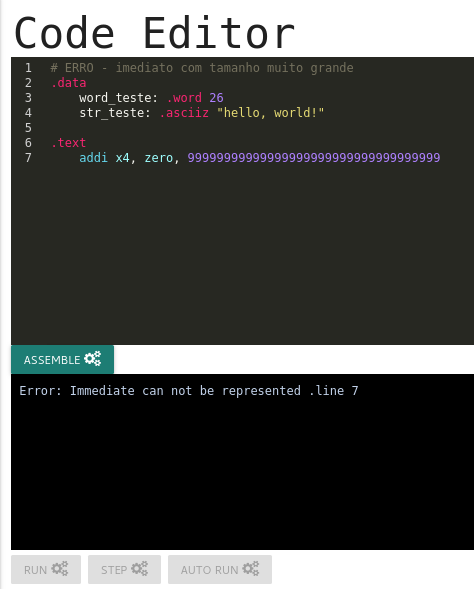
\includegraphics[width=8cm]{img/assemble_error_imediato.png}
	  \caption{Erro de imediato para o tamanho 32 de palavra 32 bits.}
	  \label{fig:assemble_error_imediato}
	\end{figure}
	 Na figura \ref{fig:assemble_error_operando_invalido}, temos um exemplo de erro de operando inválido, a instrução ADDI pede um imediato como último argumento, porém é fornecido um registrador.
	
	\begin{figure}[h!]
	  \centering
	  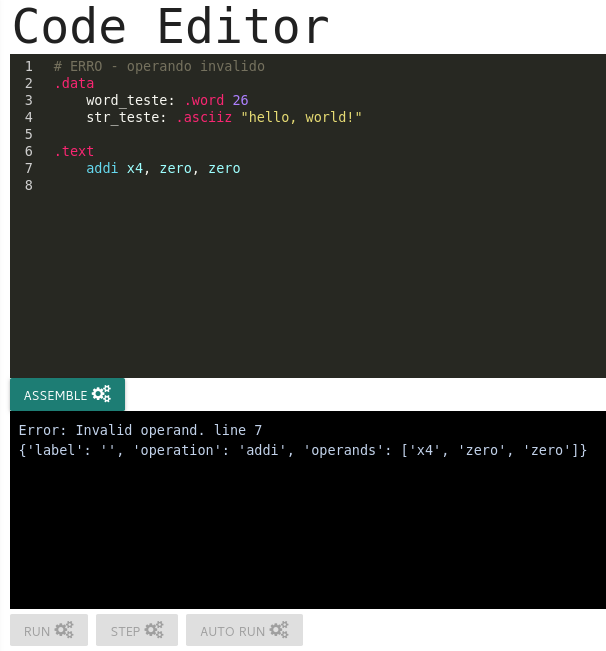
\includegraphics[width=8cm]{img/assemble_error_operando_invalido.png}
	  \caption{Erro de operando inválida, operando de tipo diferente do esperado.}
	  \label{fig:assemble_error_operando_invalido}
	\end{figure}

	 Nas figuras \ref{fig:assemble_error_operation_not_recognized}, e \ref{fig:assemble_error_op_not_recog_directives}, temos um exemplo de erro de operação não reconhecida, sendo que o primeiro mostra que foi fornecido uma instrução desconhecida, e no segundo uma diretiva desconhecida.

	\begin{figure}[h!]
	  \centering
	  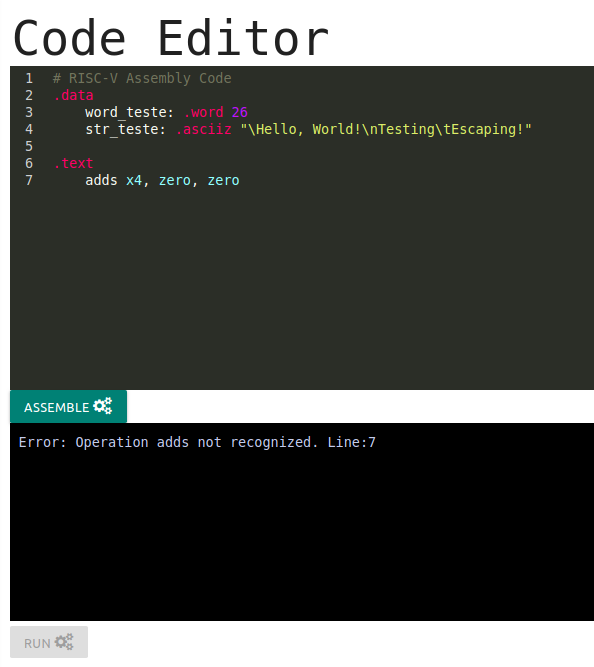
\includegraphics[width=8cm]{img/assemble_error_operation_not_recognized.png}
	  \caption{Erro de operação inválida, instrução não existente na arquitetura implementada.}
	  \label{fig:assemble_error_operation_not_recognized}
	\end{figure}

	\begin{figure}[h!]
	  \centering
	  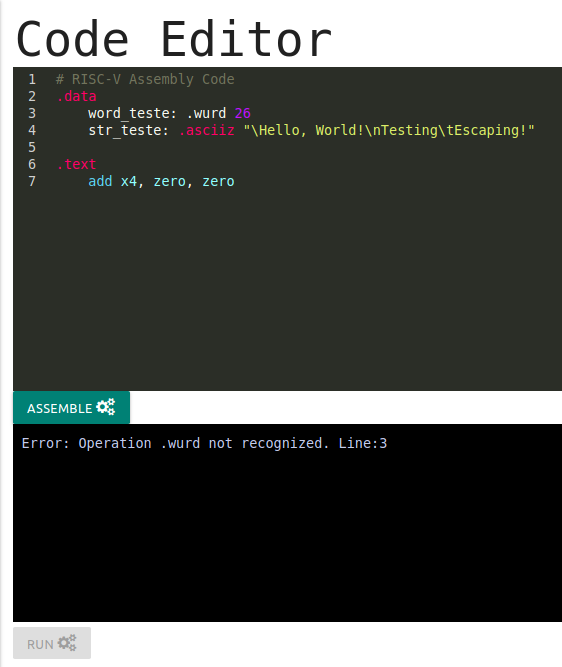
\includegraphics[width=8cm]{img/assemble_error_op_not_recog_directives.png}
	  \caption{Erro de operação inválida, diretiva não existente na arquitetura implementada.}
	  \label{fig:assemble_error_op_not_recog_directives}
	\end{figure}

	 Na figura \ref{fig:assemble_error_simbolo_inexistente}, temos um exemplo de erro de símbolo inexistente, o programador tentou utilizar um símbolo que não foi declarado antes.
	\begin{figure}[!]
	  \centering
	  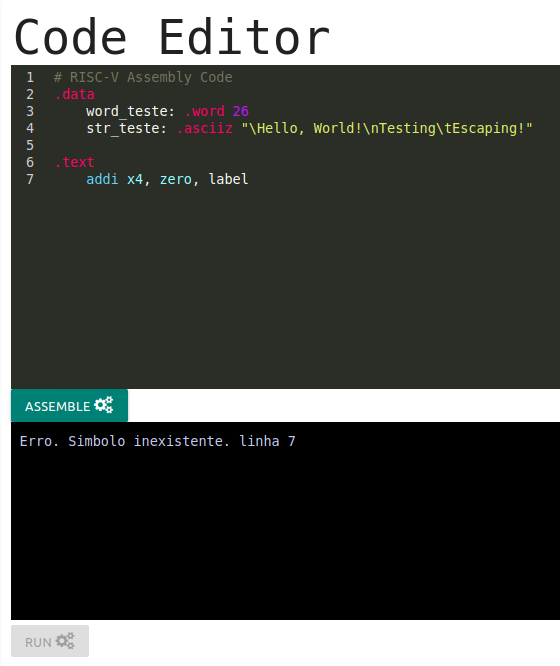
\includegraphics[width=8cm]{img/assemble_error_simbolo_inexistente.png}
	  \caption{Erro de símbolo inválido, símbolo não foi declarado.}
	  \label{fig:assemble_error_simbolo_inexistente}
	\end{figure}

	 Na figura \ref{fig:assemble_error_wrong_arguments}, temos um exemplo de erro de tipo ou número de argumentos de diretiva, parecido com o erro da figura \ref{fig:assemble_error_directives_strings}. Neste exemplo a diretiva .word pede um número e lhe é fornecido outra label.

	\begin{figure}[h!]
	  \centering
	  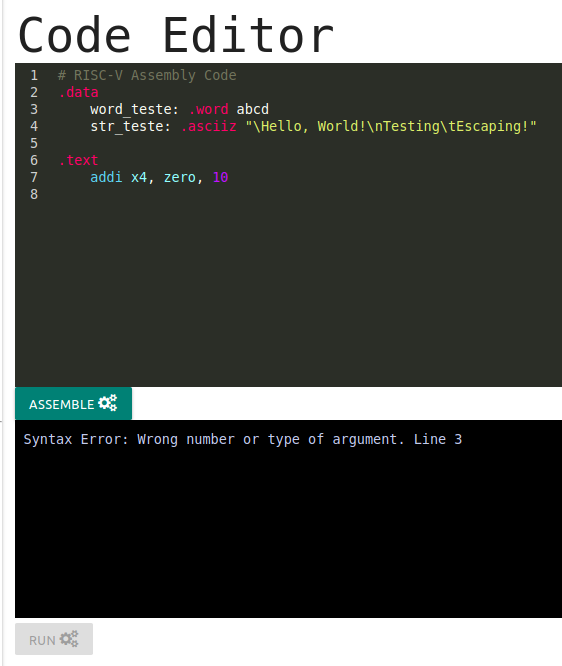
\includegraphics[width=8cm]{img/assemble_error_wrong_arguments.png}
	  \caption{Erro de argumentos de diretiva inválido, o tipo ou número de argumentos está incorreto.}
	  \label{fig:assemble_error_wrong_arguments}
	\end{figure}




\section{Aritmética Simples}
	
	Este código mostra algumas instruções matemáticas básicas, de registrador para registrador, muito utilizadas em uma variedade de programas. Neste código poderemos ver a utilização destas instruções e seus resultados em cada registrador separado, verificando suas funcionalidades.

\subsection{Editor de código}


	Na figura \ref{fig:operacoes_matematicas_codigo} está o código que utilizamos para demonstração de algumas das instruções matemáticas mais básicas. Neste exemplo foi utilziada a instrução ADDI para inicializar valores nos registradores x3 e x4. A partir dos valores contidos nestes registradores realizamos várias operações matemáticas, ADD (adição), SUB (subtração), SRL (shift right logical), SLL (shift left logical), AND, OR, XOR, SLT (set less than). 

	\begin{figure}[h]
	  \centering
	  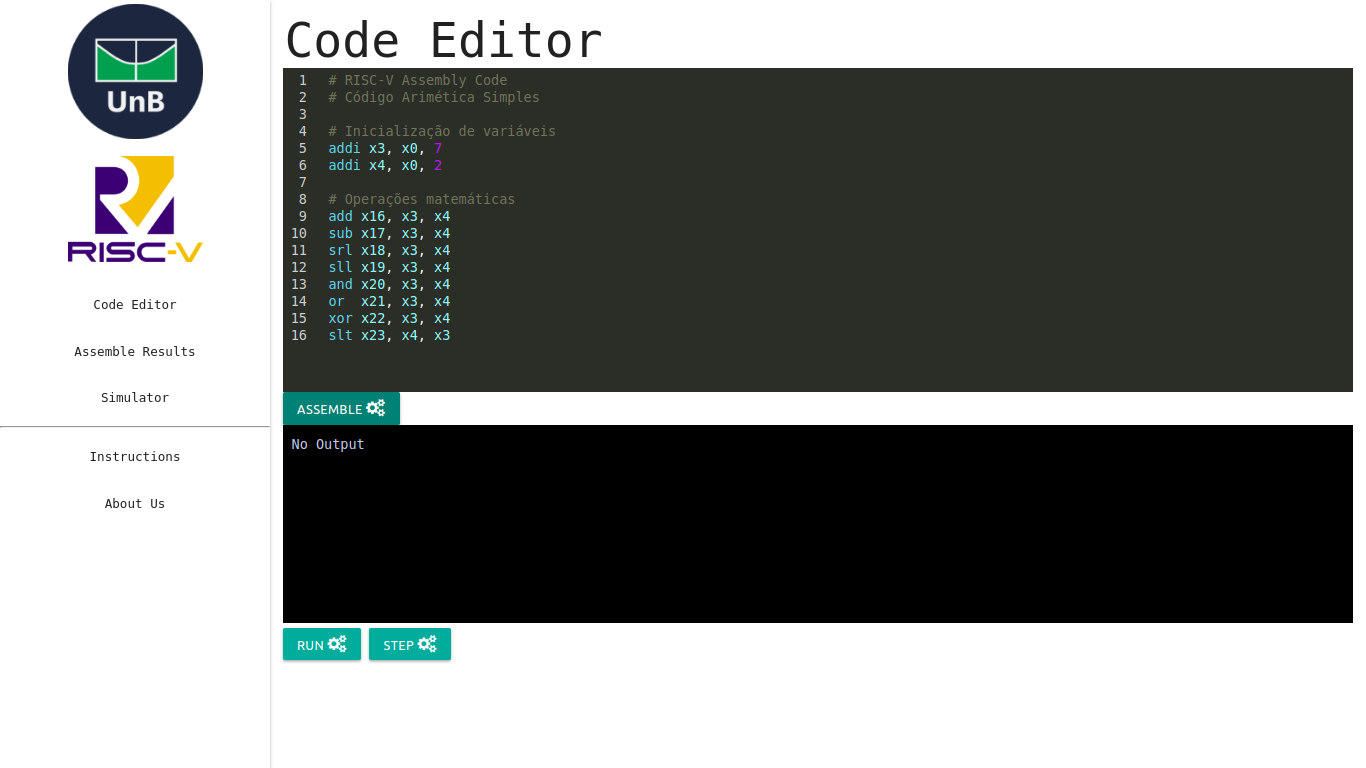
\includegraphics[width=8cm]{img/aritmetica_codigo.png}
	  \caption{Demonstração de operações matemáticas básicas.}
	  \label{fig:operacoes_matematicas_codigo}
	\end{figure}


\subsection{Simulação}
	
	Para cada operação realizada com estes valores, cada resultado foi armazenado em um registrador do x16 ao x23, como podemos ver na figura \ref{fig:operacoes_matematicas_resultados}

	\begin{figure}[h]
	  \centering
	  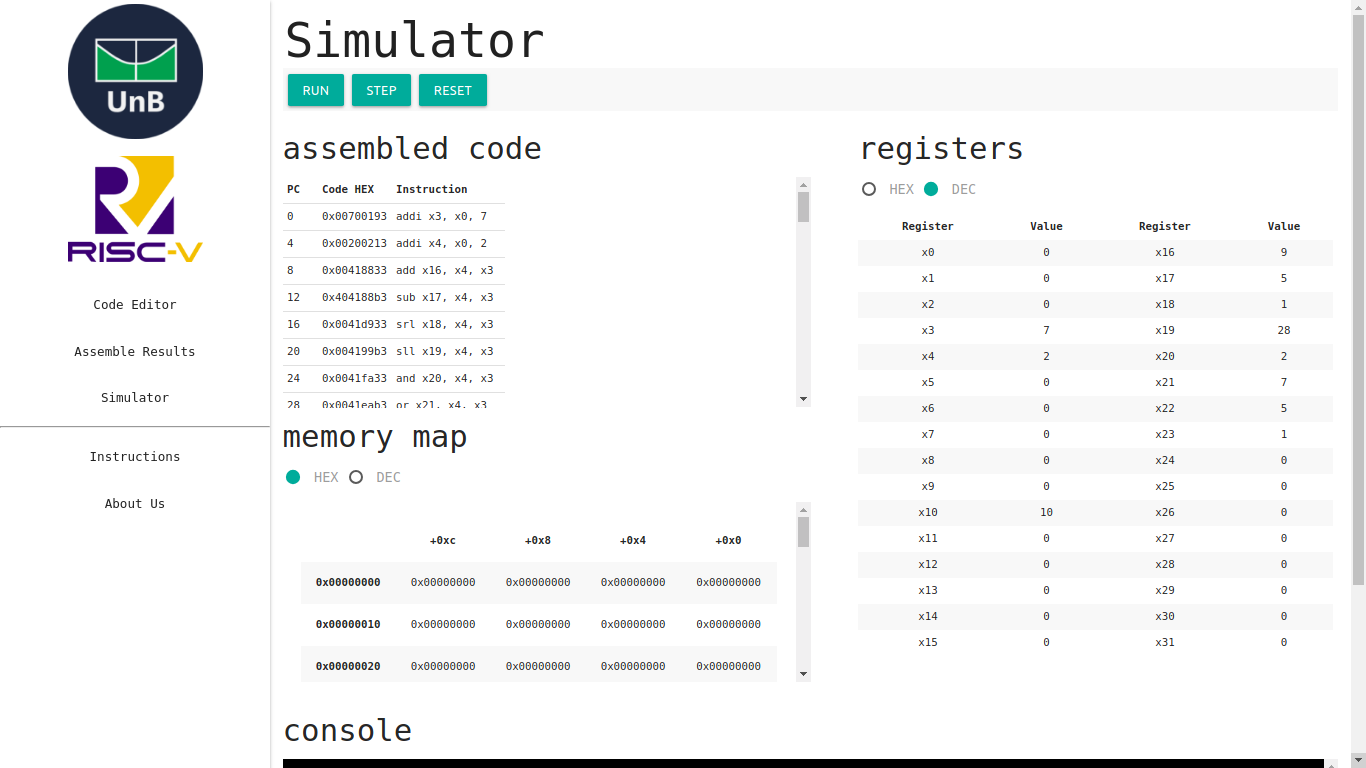
\includegraphics[width=8cm]{img/aritmetica_results.png}
	  \caption{Demonstração de operações matemáticas básicas.}
	  \label{fig:operacoes_matematicas_resultados}
	\end{figure}

	Como o programa não escreve na memória ou imprime resultados na tela, os resultados importantes a serem ressaltados são os valores de registradores e também o código montado. Os valores dos registradores são mostrados na forma decimal para visualização.


\section{Sequência de Fibonacci}
	
	A sequência de fibonacci é um dos primeiros algoritmos que aprendemos quando iniciamos nos estudos de programação. Cada termo desta sucessão de números é gerada pela soma dos dois números antescedentes.

\subsection{Editor de código}


	Na figura \ref{fig:fib-codigo-1} temos a inicialização de duas variáveis, n\textunderscore fibs, que é a quantidade de termos da sequência que desejamos obter. E a outra variável é a fib\textunderscore base\textunderscore mem\textunderscore addr. O valor atribuido a esta variável não é relevante neste programa, apenas denota a base de endereço onde serão armazenados os termos.

	Depois temos a função fib, que inicializa registradores. Colocando em x3 como o número de termos que serão escritos. Em x4 o primeiro termo de fibonacci. E em x6 um valor auxiliar. Em x10 atribuimos o valor 1 para chamadas de impressão de inteiros através de syscalls 

	Ainda podemos ver uma parte da função loop, que irá calcular novos termos. A primeira instrução BEQ serve para verificarmos se já atingimos o número de termos desejados. Após a verificação faz-se um salto para funções de impressão. Vemos também a utilização do registrador x7, que servirá de auxiliar para não perdemos o valor de atual do termo de fibonacci. E então o registrador x4 recebendo a soma do próprio x4 que é o valor atual do termo de fibonacci e x6 que é o valor auxiliar.

	\begin{figure}[h!]
	  \centering
	  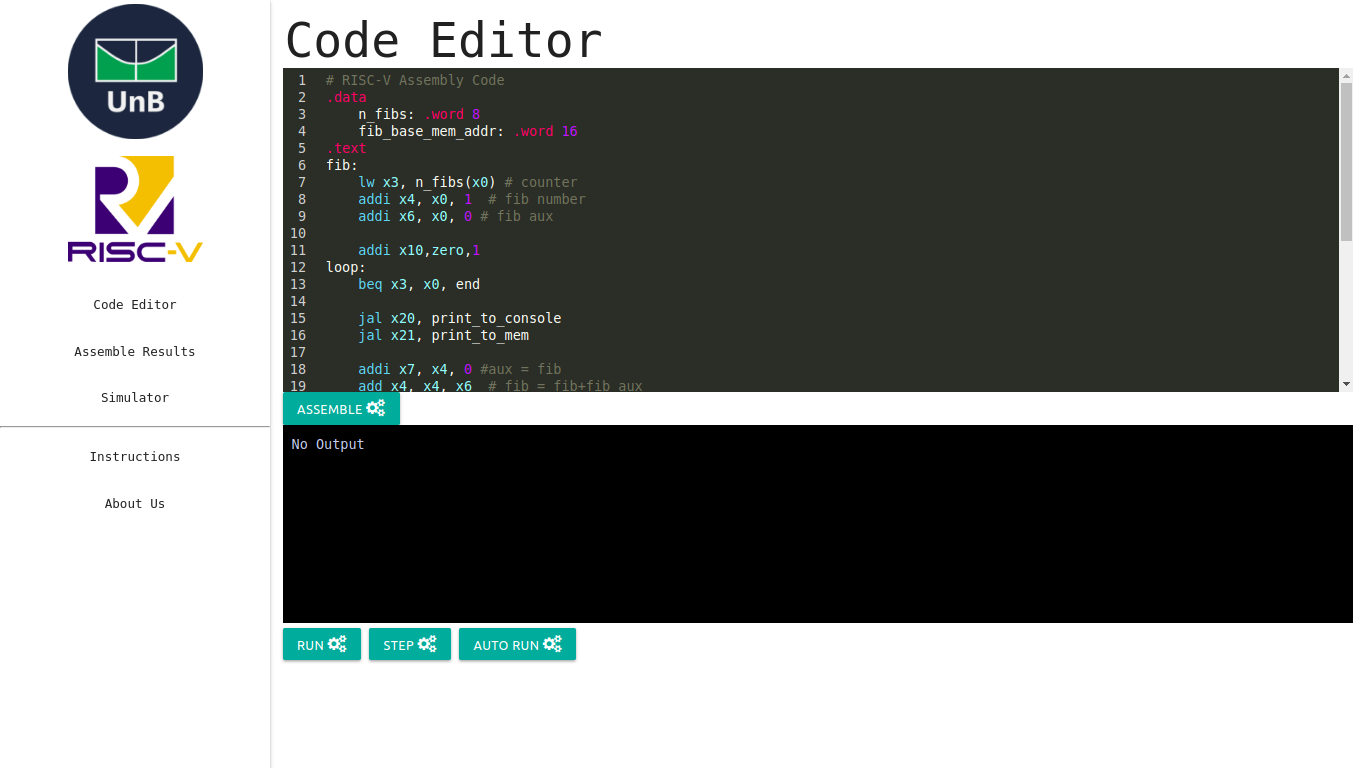
\includegraphics[width=14cm]{img/fibonacci_codigo_1.png}
	  \caption{Primeira parte do código que gera sequência de fibonacci.}
	  \label{fig:fib-codigo-1}
	\end{figure}

	Na continuação da função loop, mostrado na figura \ref{fig:fib-codigo-2}, somamos o valor em x7, valor do termo anterior, com 0 e adicionamos em x6, variável auxiliar de fibonacci.

	Após encontrar os termos terem sido atualizados para o pŕoximo laço se faz um decremento do valor do registrador x3, que contém a quantidade de termos que o usuário deseja, que foi obtido a partir da label n\textunderscore fibs.

	Depois de decrementado o valor, se faz um salto para o início do loop, onde vai ser verificado se já foram encontrados todos os valores desejados e se pode pular para a label end e encerrar o programa. 

	Em seguida, nas linhas 25 e 30, estão as labels para as chamadas das rotinas de impressão chamadas dentro da função loop, print\textunderscore to\textunderscore console, e print\textunderscore to\textunderscore mem. Estas rotinas não utilizam a pilha para variáveis e retornos, como se utilizassem apenas variáveis gloabais.

	A função print\textunderscore to\textunderscore console simplesmente mvoe o valor de x4, termo de fibonacci, para o registrador x5, que é utilizado dentro da instrução ECALL (environment call). E então retornamos ao loop com a instrução JALR.

	A outra função, print\textunderscore to\textunderscore mem, faz um SW (store word) do valor contido no registrador x4 no endereço dado pela soma do valor de x30 adicionado do endereço da variável de fib\textunderscore base\textunderscore mem\textunderscore addr. Depois adicionamos 4 em x30 para que no próximo laço seja impresso o próximo inteiro no endereço de store word correto. E então retornamos ao loop.

	\begin{figure}[h]
	  \centering
	  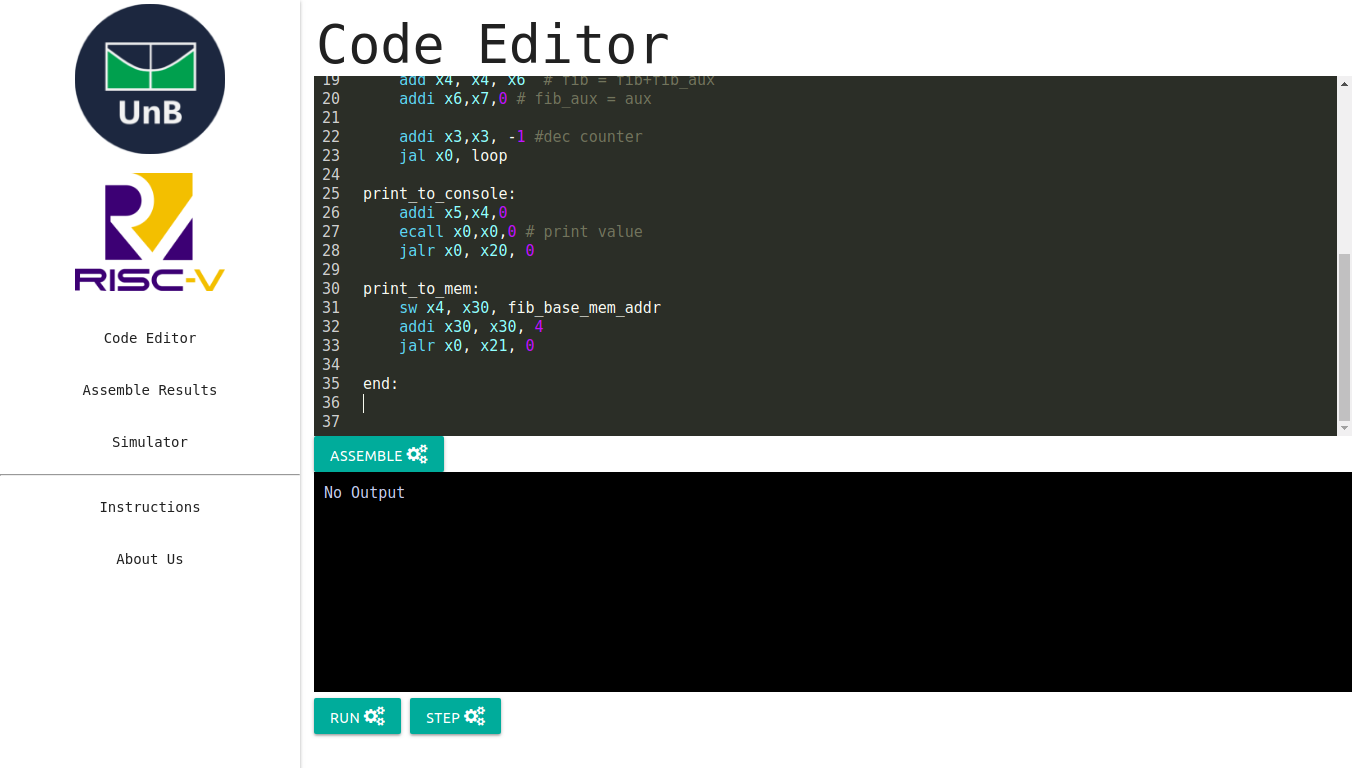
\includegraphics[width=14cm]{img/fibonacci_codigo_2.png}
	  \caption{Segunda parte do código que gera sequência de fibonacci.}
	  \label{fig:fib-codigo-2}
	\end{figure}

	Ao final do código devemos ter o número de termos de fibonacci fornecidos pelo usuário mostrado tanto na console de saída quanto em endereços na memória.



\subsection{Simulação}

	
	Na primeira parte dos resultados demonstrados na figura \ref{fig:fib-results-1} vemos parcialemnte o código montado gerado pelo montador, valores residuais dos registradores utilizados e os valores da memória.

	\begin{figure}[h]
	  \centering
	  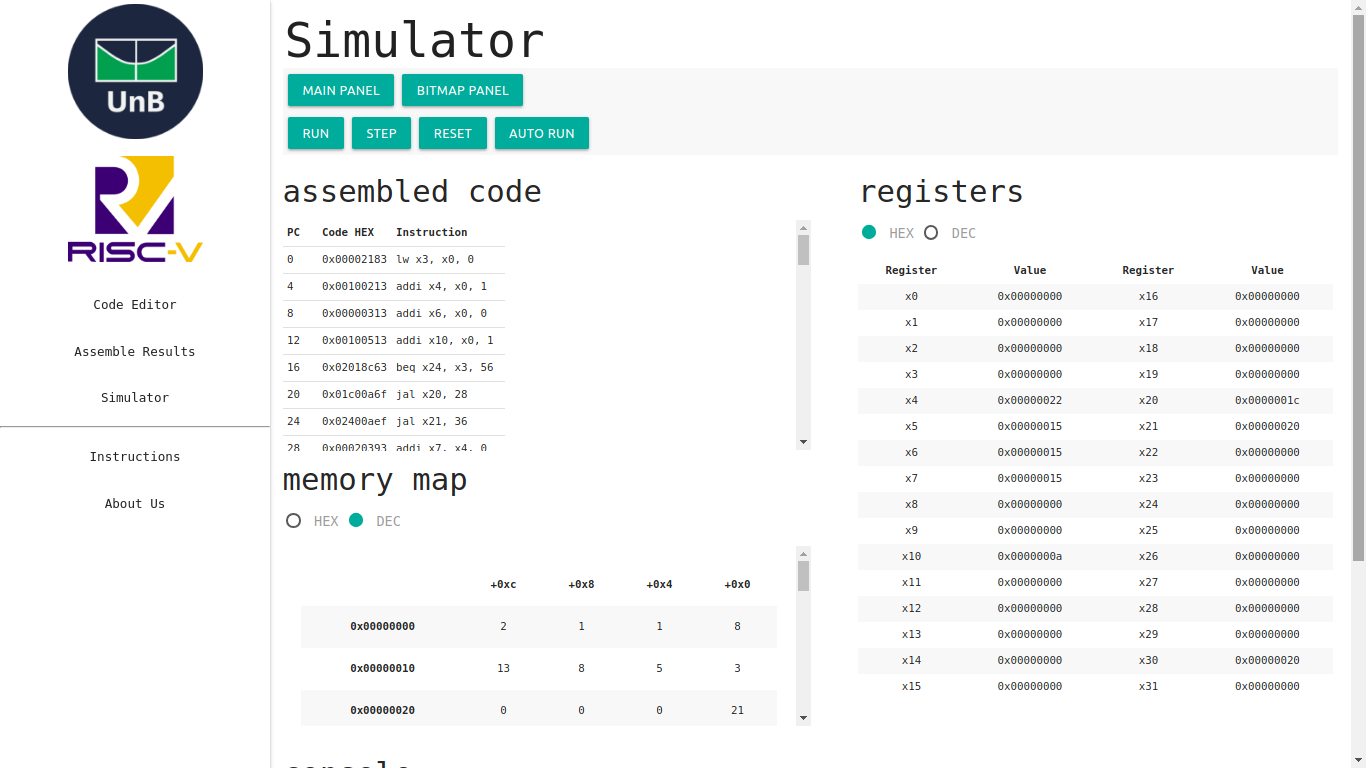
\includegraphics[width=14cm]{img/fibonacci_results_1.png}
	  \caption{Primeira parte dos resultados gerados da sequência de fibonacci.}
	  \label{fig:fib-results-1}
	\end{figure}

	Na primeira instrução vemos que o programa executa um Load Word no endereço 0 da memória, este endereço contém o valor fornecido pelo programador com o número de termos de fibonacci gue gostaria de obter. A partir do segundo endereço, o 0x00000004, temos a sequência de valores de fibonacci impressos na memória a cada iteração do loop.

	Na figura \ref{fig:fib-results-2} podemos ver a console de saída. Esta parte nos mostra a funcionalidade da chamada de ambiente, ou SYSCALL, que imprime um número inteiro na tela. 

	\begin{figure}[h]
	  \centering
	  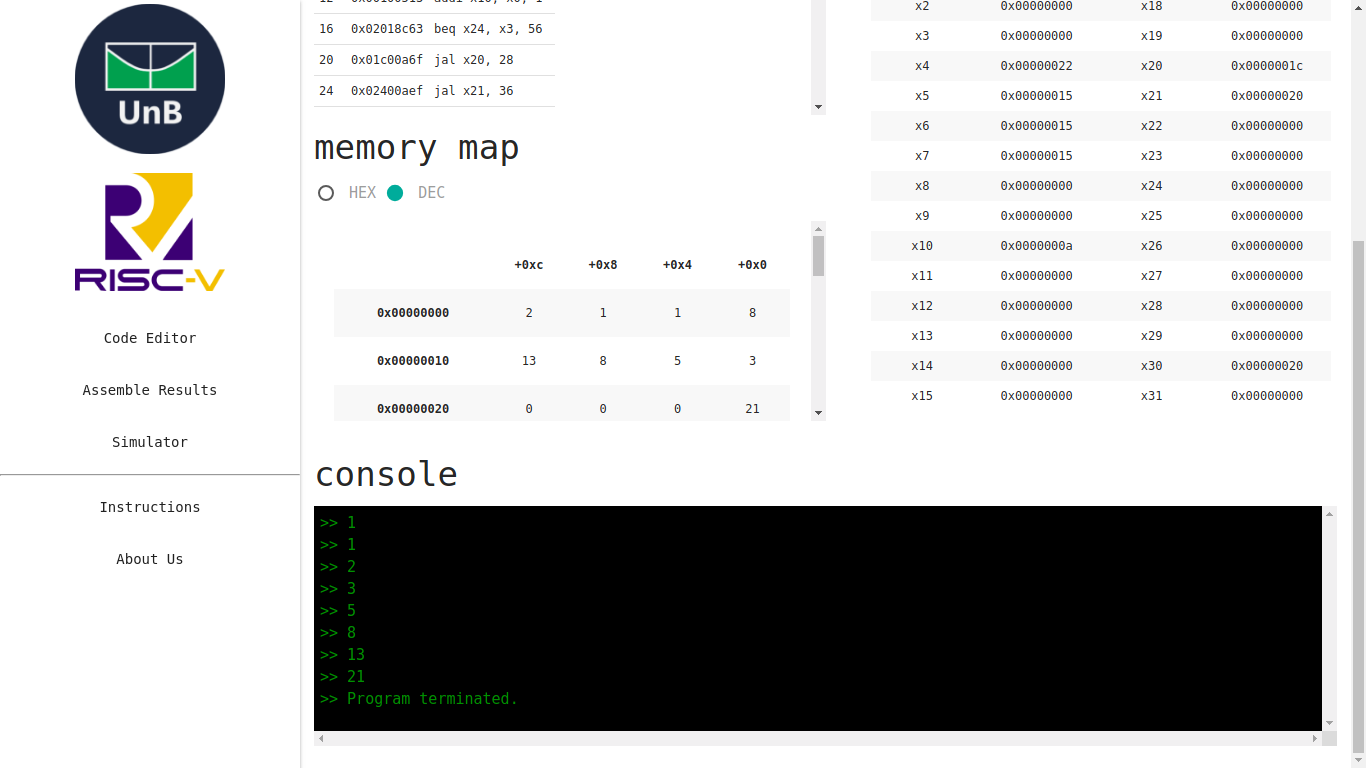
\includegraphics[width=14cm]{img/fibonacci_results_2.png}
	  \caption{Segunda parte dos resultados gerados da sequência de fibonacci.}
	  \label{fig:fib-results-2}
	\end{figure}

	Os termos foram impressos um em cada linha, cada linha representa uma chamada da instrução ECALL com o valor 1 no registrador x10, e o termo a ser impresso contido no registrador x5. E ao final do código temos a outra chamada de ambiente implementada que é a de saída do programa, chamando ECALL com o valor 10 no registrador x10.

